\section{Results Analysis}

\subsection{\tt interpolateTemperature}

The built-in function allows to interpolate temperature in thermal result at arbitrary spatial locations. \\

\renewcommand{\arraystretch}{1.5}
\begin{table}[h]
    \centering
    \begin{tabular}{|>{\customfont}c|>{\customfont}c|>{\customfont}c|}
        \hline 
        \rowcolor{gray!30}
        \textbf{Fields} & \textbf{Type} & \textbf{Description} \\ \hline
        \tt thermalResults & \tt TransientThermalResults & results of the simulation returned by \texttt{Simulate} \\ \hline 
        \tt querypoints & \tt double & coordinates specified as a vector \\ \hline 
    \end{tabular}
\end{table}



\textbf{Example :} interpolates temperature at the origin of geometry

\begin{lstlisting}[language=Matlab]
simulation=Simulate(geometry, options);
tempOrigin=interpolateTemperature(simulation,[0;0;0],1:numel(simulation.SolutionTimes));
\end{lstlisting}
\ 


\subsection{Built-in visualization tools} 

The {\tt geometryView} function allows the user to save the following figures of the geometry in a pdf file.\\
One can call the function in a script using: 

\begin{lstlisting}[language=Matlab]
tools.geometryView('Geometry.pdf', simulation, geometry);
\end{lstlisting}

It saves in a file the three following figures:\\

\textbf{\tt pdeplot3D} : Plot solution or surface mesh for 3-D problem.

\begin{lstlisting}[language=Matlab]
simulation=Simulate(geometry, options);
figure;
pdeplot3D(simulation.Mesh,ColorMapData=simulation.Temperature(:,end));
\end{lstlisting}

\begin{center}
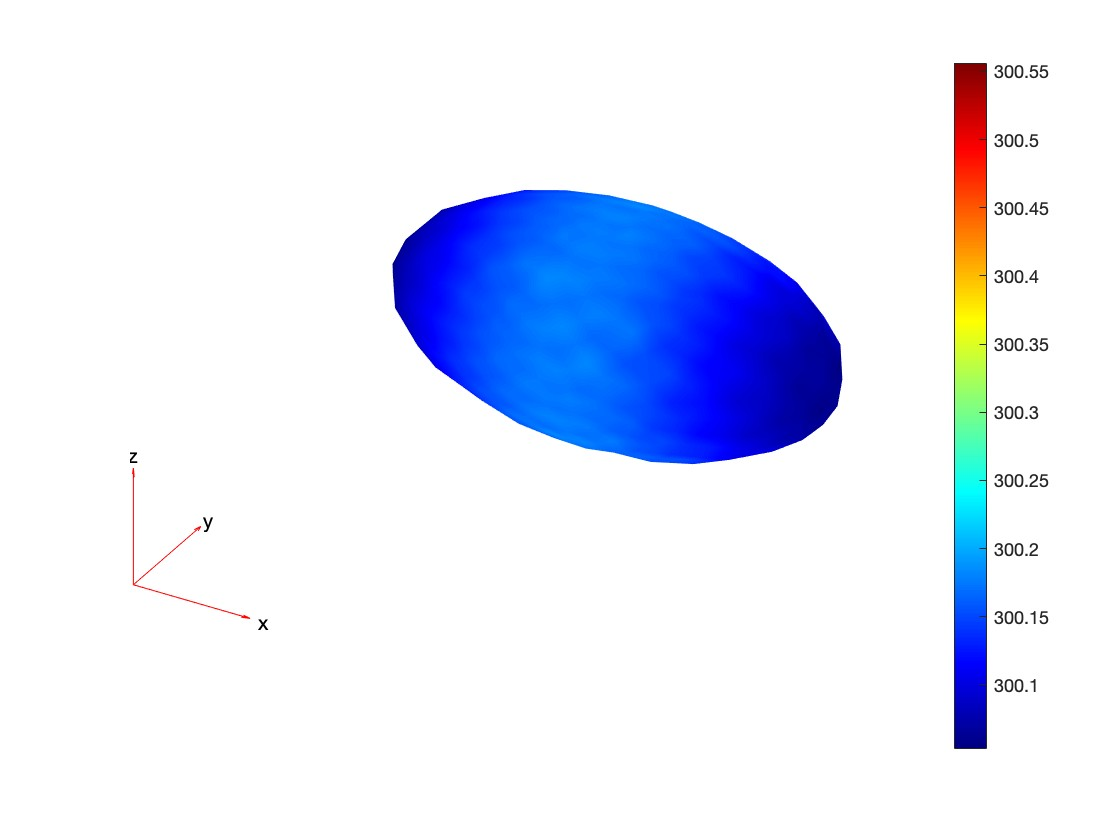
\includegraphics[scale=0.18]{Example/pdeplot3D.jpg}
\end{center}


\textbf{\tt pdegplot} : Plot PDE geometry. 

\begin{lstlisting}[language=Matlab]
figure;
pdegplot(geometry.structure, "FaceAlpha",0.2);
\end{lstlisting}

\begin{center}
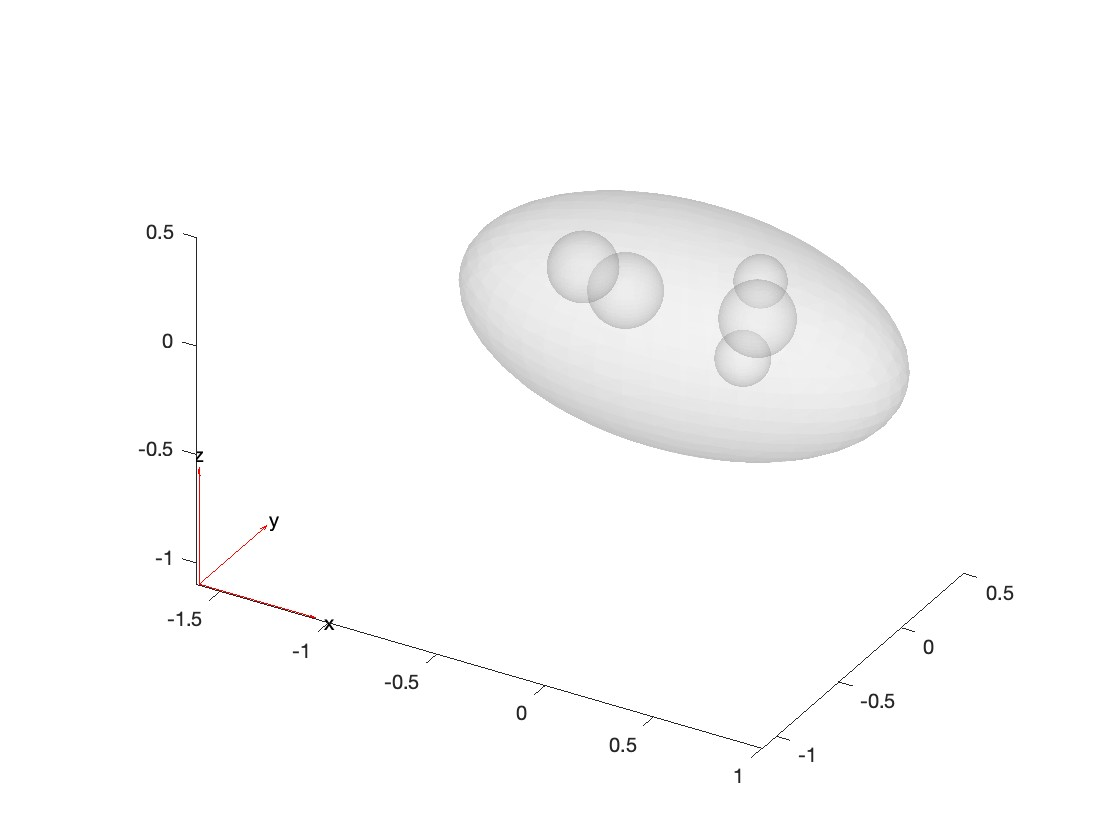
\includegraphics[scale=0.18]{Example/pdegplot.jpg}
\end{center}


\textbf{\tt pdemesh} : Plot PDE mesh.\\

\begin{lstlisting}[language=Matlab]
simulation=Simulate(geometry, options);
figure;
pdemesh(simulation.Mesh);
\end{lstlisting}
\ 

\begin{center}
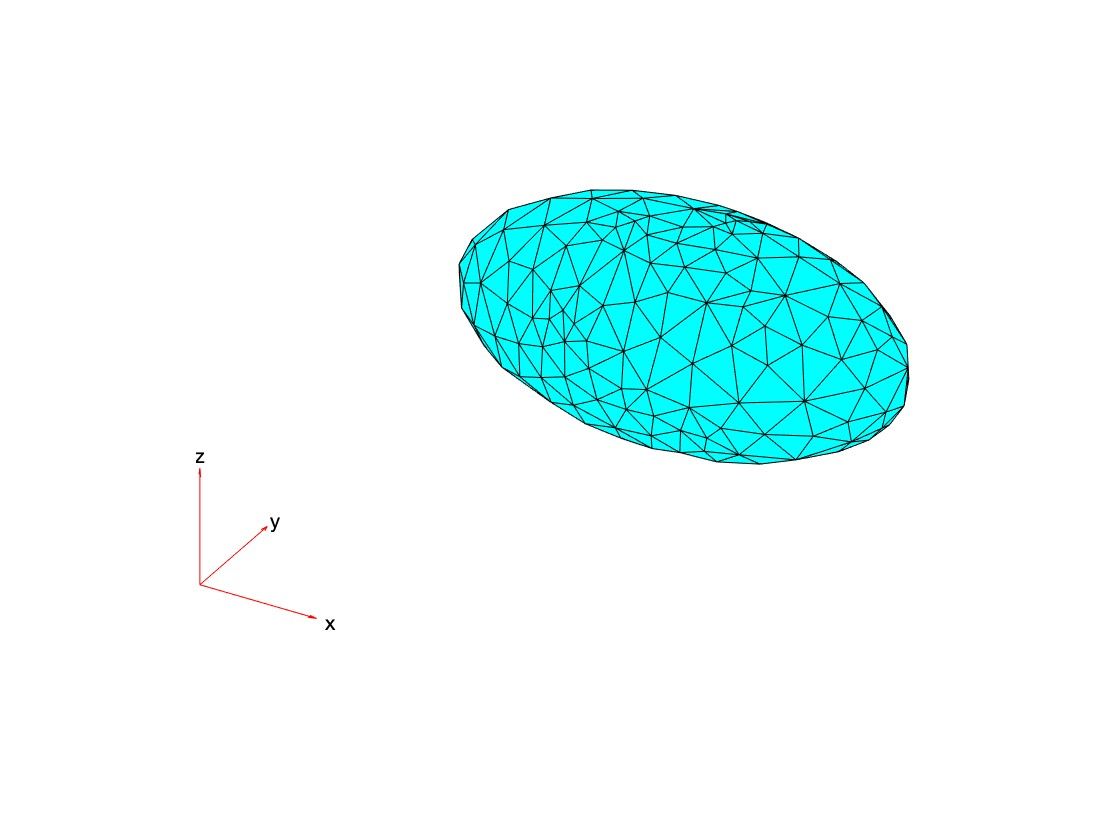
\includegraphics[scale=0.25]{Example/pdemesh.jpg}
\end{center}
\ 



\subsection{Isosurface 3D animation}

One can create an animation of the thermal evolution at a given temperature. The {\tt isosurface} function hence export the animation in a video file. Parameters are the video filename, the result structure of the simulation, and a temperature to render the isosurface. \\

\textbf{Example :} Animation of a cube with voided cavities at Curie temperature

\begin{lstlisting}[language=Matlab]
tools.isosurface('Animation.avi', simulation, options.TCurie);
\end{lstlisting}
\ 


\begin{center}
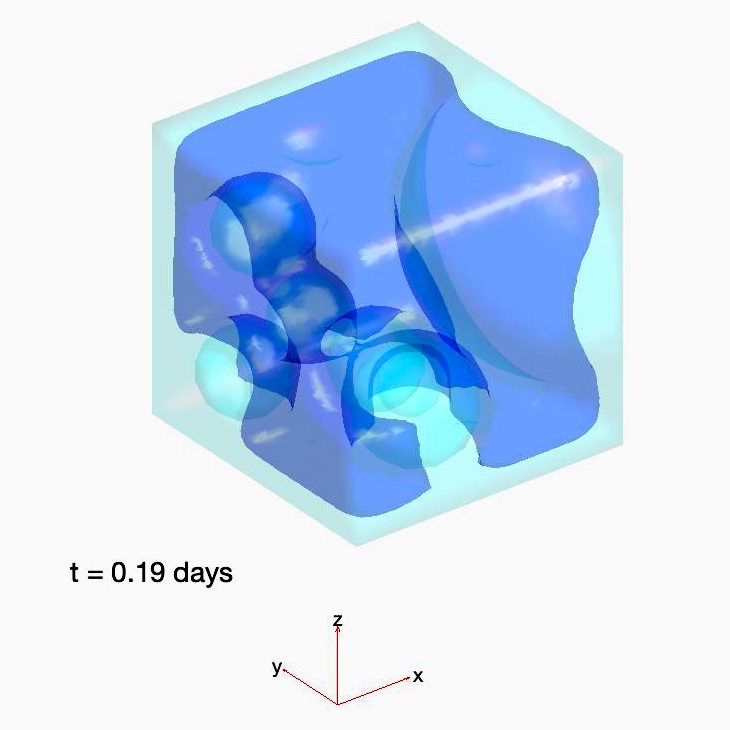
\includegraphics[scale=0.3]{Example/animation.png}
\end{center}
\ 


\newpage

\subsection{Heat map slice view}

One can represent the temperature distribution inside the geometry at different time steps, inside a chosen plane. To do so, the {\tt heatMapSlice} and {\tt heatMapSliceAnimation} functions located in the {\tt tools} folder are implemented. The first one outputs a subplot of the heatmap at different times, whereas the second outputs an animation under a video file. They both take the following parameters 

\renewcommand{\arraystretch}{1.5}
\begin{table}[h]
    \centering
    \begin{tabular}{|>{\ttfamily}c|>{\ttfamily}c|>{\raggedright\arraybackslash}p{8cm}|}
        \hline 
        \rowcolor{gray!30}
        \textbf{Fields} & \textbf{Type} & \textbf{Description} \\ \hline
        filename & string & Filename under which to save the figure or animation (\texttt{.pdf} or \texttt{.avi}) \\ \hline
        thermalResults & TransientThermalResults & Results of the simulation returned by \texttt{Simulate} \\ \hline 
        view\_type & string & Slice plane for representation; must be \texttt{'x'}, \texttt{'y'}, or \texttt{'z'} \\ \hline 
        value & double & Value of the slice view plane \\ \hline 
    \end{tabular}
\end{table}

\medskip

\textbf{Example :} One can obtain the visualization in the $z=0$ plane by calling the function

\begin{lstlisting}[language=Matlab]
tools.heatMapSlice('slice.pdf',simulation,'z',0);
tools.heatMapSliceAnimation('sliceAnimation.avi',simulation,'z',0);
\end{lstlisting}

\medskip
Considering the following geometry with low thermal diffusivity in heterogeneous material :

\begin{center}
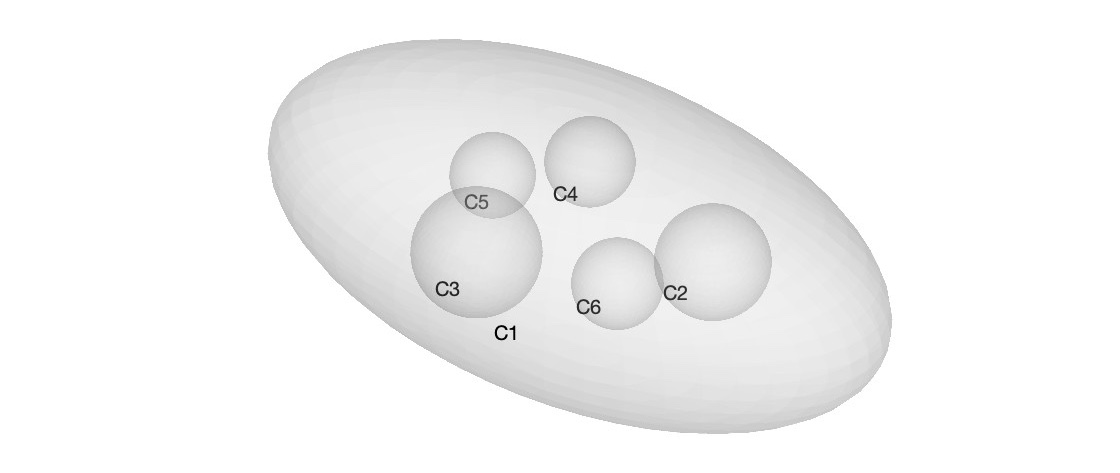
\includegraphics[scale=0.2]{Example/example2_gm.jpg}
\end{center}

With the {\tt heatMapSlice} function, one can get 
\begin{center}
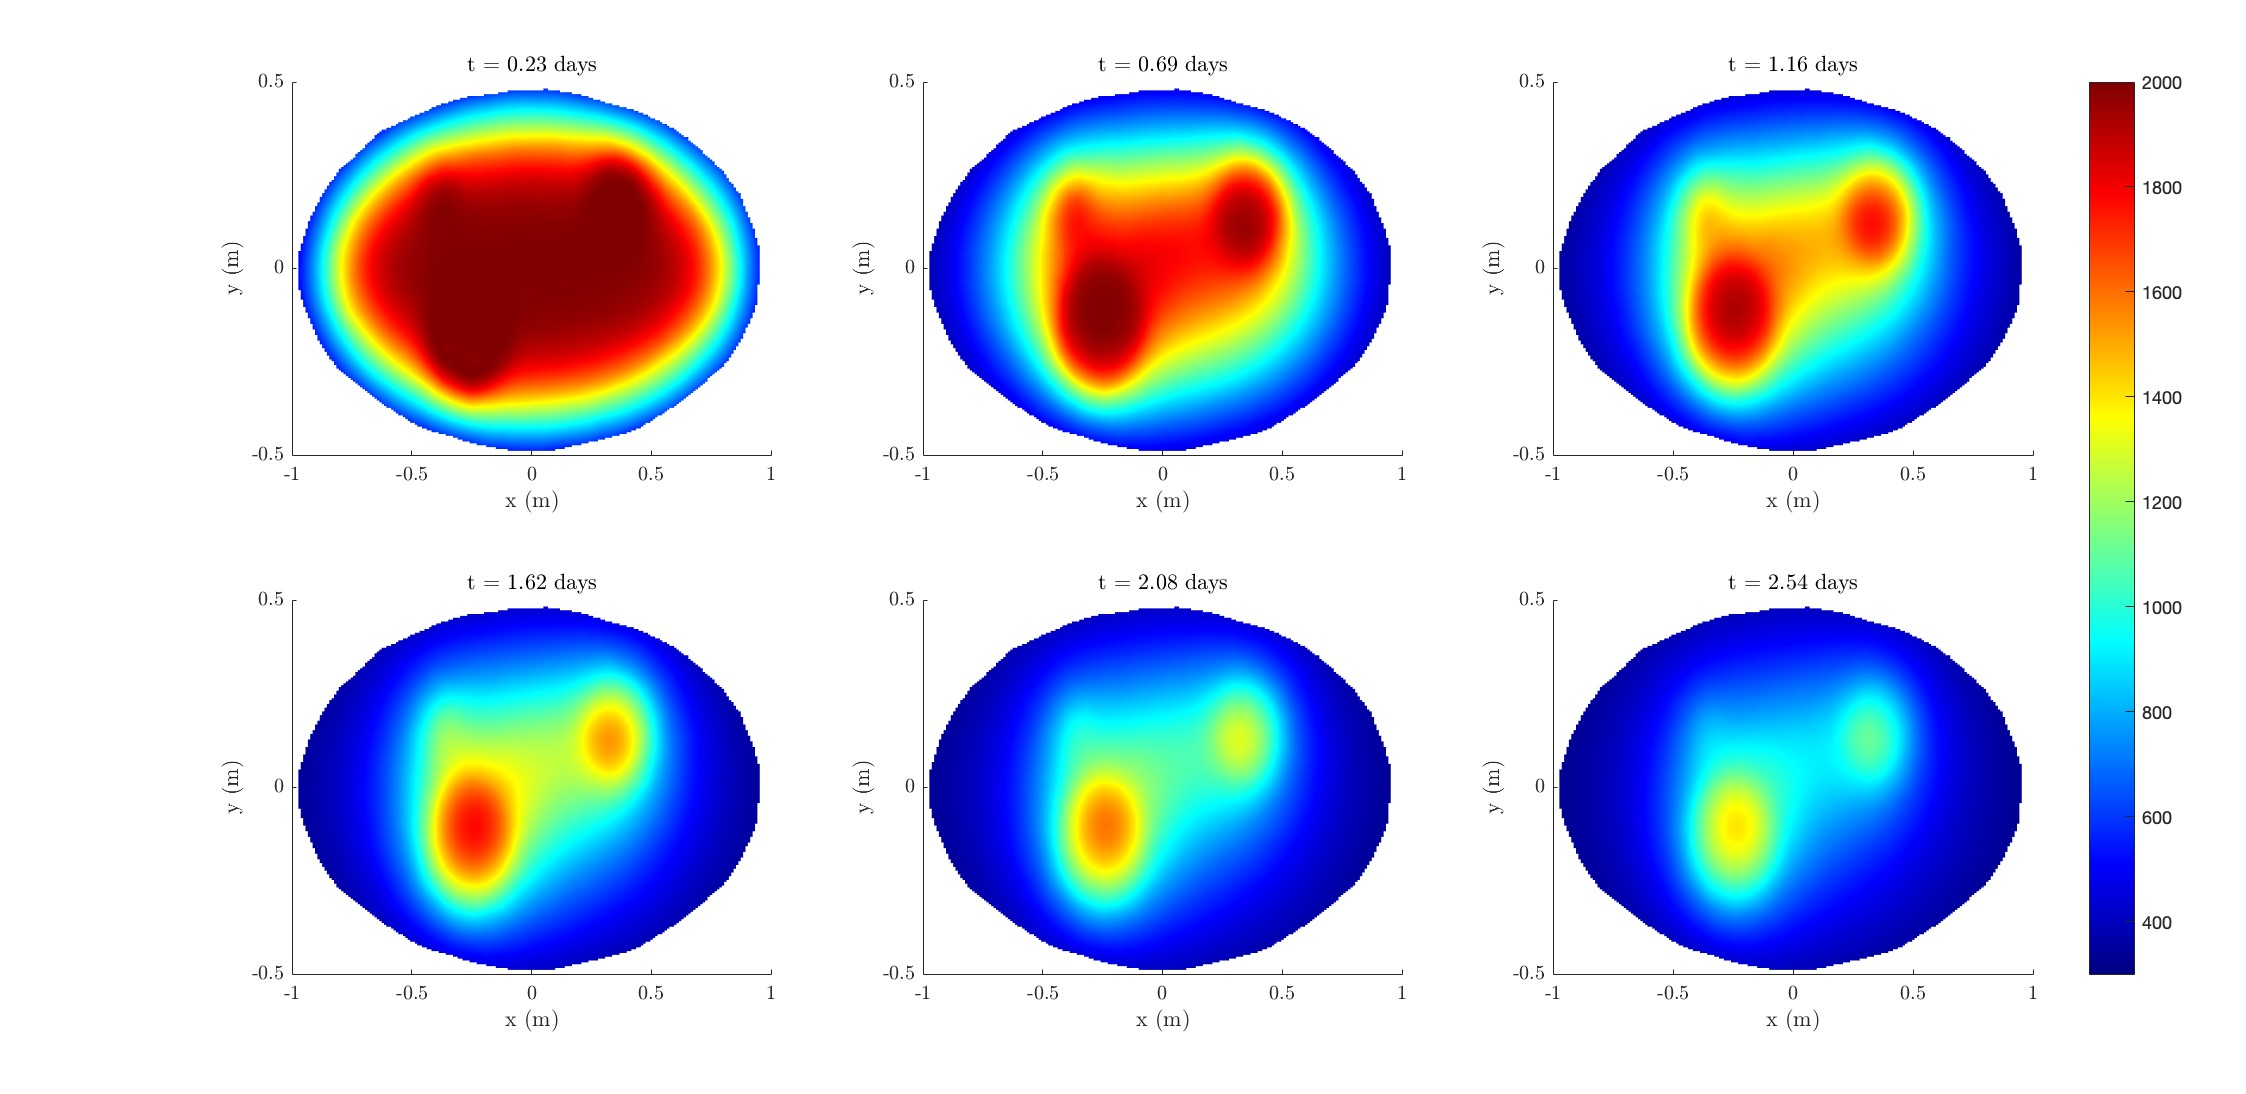
\includegraphics[scale=0.2]{Example/example2_slice.jpg}
\end{center}